\documentclass{beamer}
\usetheme{Boadilla}

\usepackage{amsmath}
\usepackage{amsfonts}
\usepackage{hyperref}
\usepackage{algorithm}
\usepackage{algpseudocode}


\usepackage{amsmath}
\DeclareMathOperator*{\argmax}{arg\,max}
\DeclareMathOperator*{\argmin}{arg\,min}

\title{How To Train Your MAML}
\author{Dmitry Protasov}
\institute{MIPT}

\begin{document}

\begin{frame}
    \titlepage
\end{frame}

% \begin{frame}
%     \tableofcontents
% \end{frame}

\section{Introduction}
\begin{frame}{Introduction to Meta-Learning}
    \begin{block}{Few-shot Learning and Meta-Learning}
        \begin{itemize}
            \item \textit{Few-shot learning} is challenging without prior knowledge; \textit{meta-learning} automates the acquisition of \textit{across-task knowledge}.
            \item \textit{Meta-learning}: Models learn to rapidly assimilate \textit{task-specific knowledge} from limited data, enhancing learning proficiency with experience.
            \item \textit{MAML's} simplicity and adaptability make it a meta-learning framework that achieves state-of-the-art results.
        \end{itemize}
    \end{block}
\end{frame}

\section{Background}
\begin{frame}{Related Work}
    \begin{block}{Key Developments in Few-Shot Learning}
        \begin{itemize}
            \item \textit{Matching Networks} use cosine distance and a differentiable embedding function to match items between support and target sets, converting distances into probability distributions over classes.
            \item \textit{Gradient-conditional meta-learner LSTM} --  learns how to update a base-learner model% , single update at inference time
            \item \textit{MAML}: increasing the gradient update steps and using Batch Stochastic Gradient Descent to speed up learning and enhance generalization. SOTA in Omniglot and Mini-Imagenet.
            \item \textit{Meta-SGD}: learns static learning rate and update direction for each parameter + initialization parameters.%, significantly improving generalization with a single inner loop update %but increasing model parameters and computational overhead.
        \end{itemize}
    \end{block}
\end{frame}

\section{Model Agnostic Meta-Learning (MAML)}
\begin{frame}{Formal Problem Setting}
    \begin{block}{Base Model and Meta-Parameters}
        We define a \textit{base model} \( f_{\theta} \) with meta-parameters \( \theta \). The goal is to learn initial parameters \( \theta_0 \) so that after \( N \) gradient updates with data from a support set \( S_b \), the model performs well on the target set \( T_b \).
    \end{block}
    \begin{block}{Inner-loop update process}
        Updated base-network parameters after \( i \) steps on data from \( S_b \) are given by:
        \[ \theta^b_i = \theta^b_{i-1} - \alpha \nabla_{\theta} \mathcal{L}_{S_b}(f_{\theta^b_{i-1}}), \]
        where \( \alpha \) is the learning rate and \( \mathcal{L}_{S_b} \) is the loss on the support set after \( i-1 \) update steps.
    \end{block}
\end{frame}
\begin{frame}{Formal Problem Setting}
    \begin{block}{Meta-objective and Outer-loop update process}
        The \textit{meta-objective}, reflecting the quality of \( \theta_0 \) across all tasks, is minimized to optimize \( \theta_0 \):
        \[ \mathcal{L}_{meta}(\theta_0) = \sum_{b=1}^B \mathcal{L}_{T_b}(f_{\theta^b_N}(\theta_0)), \]
        leading to the meta-parameter update:
        \[ \theta_0 = \theta_0 - \beta \mathcal{L}_{meta}(\theta_0) = \theta_0 - \beta \nabla_{\theta} \sum_{b=1}^B \mathcal{L}_{T_b}(f_{\theta^b_N}(\theta_0)), \]
        with \( \beta \) as the meta-learning rate and $\mathcal{L}_{T_b}$
denotes the loss on the target set for task b.
    \end{block}
\end{frame}


\begin{frame}{MAML Issues Summary}
    \begin{block}{}
        \begin{itemize}
            \item Training Instability: MAML may be unstable during training due to gradient issues exacerbated by networks without skip-connections.
            \item Second Order Derivative Cost: Computationally expensive + first-order approximations negatively impacting generalization.
            \item BatchNorm Issues: Using current batch statistics rather than accumulated statistics affects generalization performance and model stability.
            \item Fixed Biases in Batch Normalization: Inner-loop updates use the same batch normalization biases, assuming incorrectly that feature distribution remains constant.
            \item Shared Learning Rates: %A single learning rate for all parameters and steps%
            complicates hyperparameter tuning %and can be computationally expensive.
            \item Fixed Outer Loop Learning Rate: A static learning rate in the outer loop may hinder generalization and optimization, compared to annealing strategies.
        \end{itemize}
    \end{block}
\end{frame}

\section{Stable, Automated, and Improved MAML: Solutions}
\begin{frame}{Stabilizing MAML}
\begin{block}{Multi-Step Loss Optimization (MSL)}
To counteract gradient instability, we optimizе a weighted sum of losses after each update, enhancing stability and convergence.
\begin{equation}
\theta = \theta - \beta\nabla_\theta \sum_{b=1}^B \sum_{i=0}^N v_i L_{T_b}(f_{\theta^b_i})
\end{equation}
\end{block}

\begin{block}{Derivative-Order Annealing (DA)}
    \begin{itemize}{}
        \item use first-order gradients for the first 50 epochs
        \item then switch to second-order gradients (achieving the strong generalization)
    \end{itemize}
\end{block}
\begin{block}{Batch Normalization Running Statistics (BNRS)}
    Using per-step running statistics for batch normalization to improve optimization and generalization.
\end{block}
\end{frame}

\begin{frame}{Stabilizing MAML}
    \begin{block}{Per-Step Batch Normalization Weights and Biases (BNWB)}
        To fix this problem of Shared BatchNorm bias we propose learning a set of biases per-step within the inner-loop update process.
    \end{block}
    \begin{block}{Learning Per-Layer Per-Step Learning Rates and Gradient Directions (LSLR)}
        Learning rates and gradient directions for each layer and each step, reducing memory and computational load.
    \end{block}
    \begin{block}{Cosine Annealing of Meta-Optimizer Learning Rate (CA)}
        Implementing cosine annealing for the meta-optimizer's learning rate to fit training data better and enhance generalization.
    \end{block}
\end{frame}

\begin{frame}{Results}
    \begin{figure}{}
        \centering
        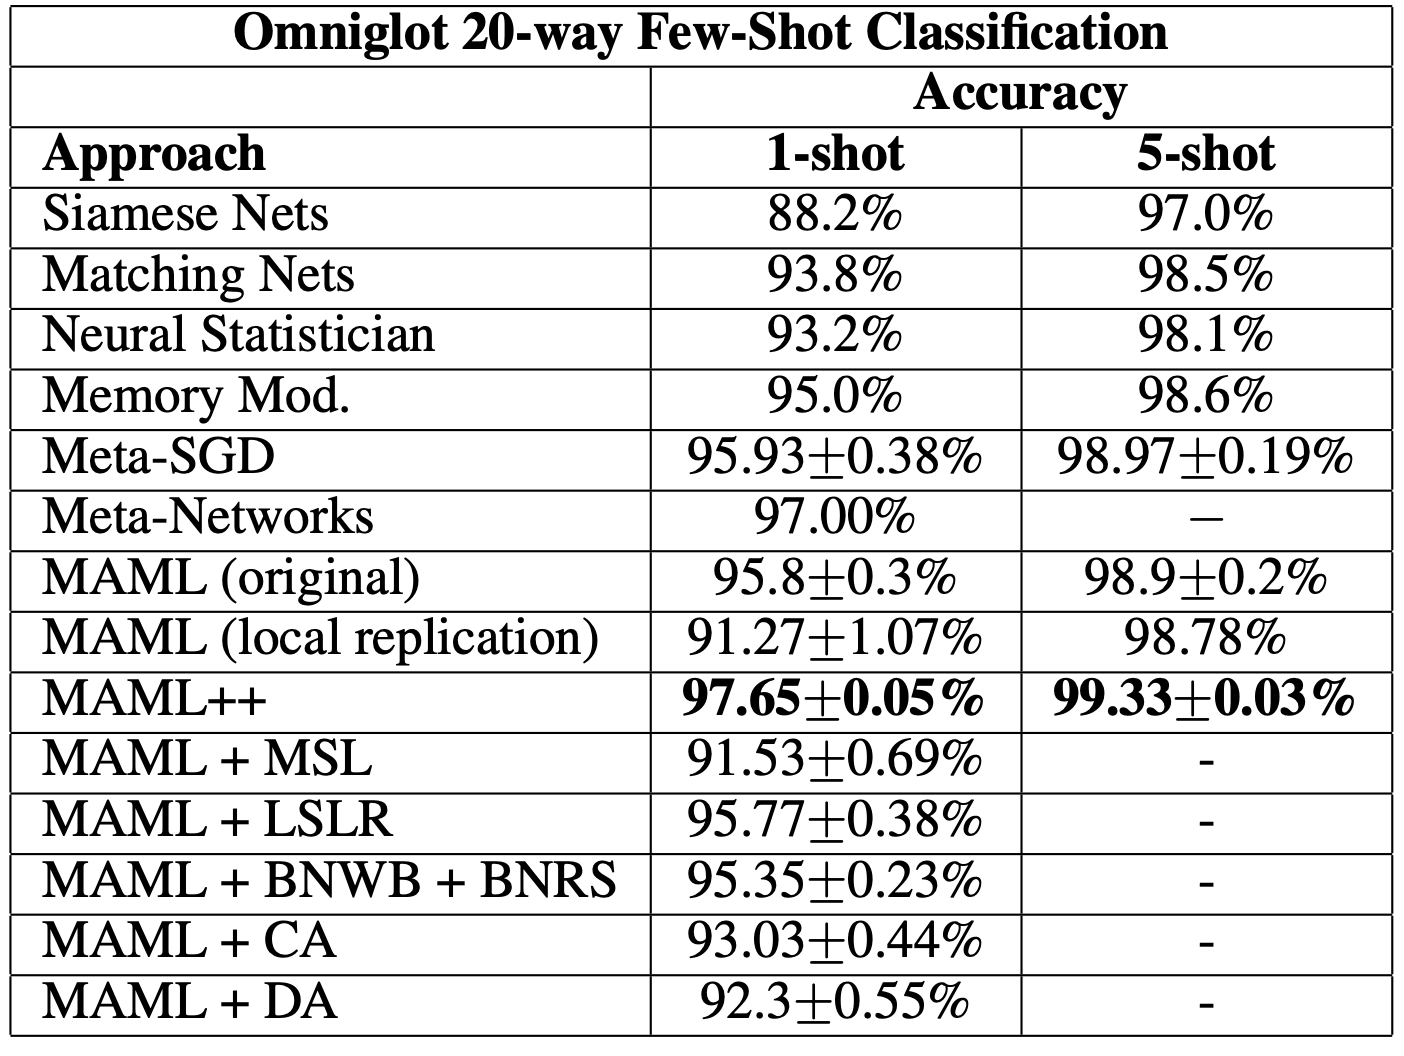
\includegraphics[scale=0.32]{images/table1.png}
        \caption{MAML++ Omniglot 20-way Few-Shot Results}
        \label{fig:enter-label}
    \end{figure}
\end{frame}

\begin{frame}{Results}
    \begin{figure}{}
        \centering
        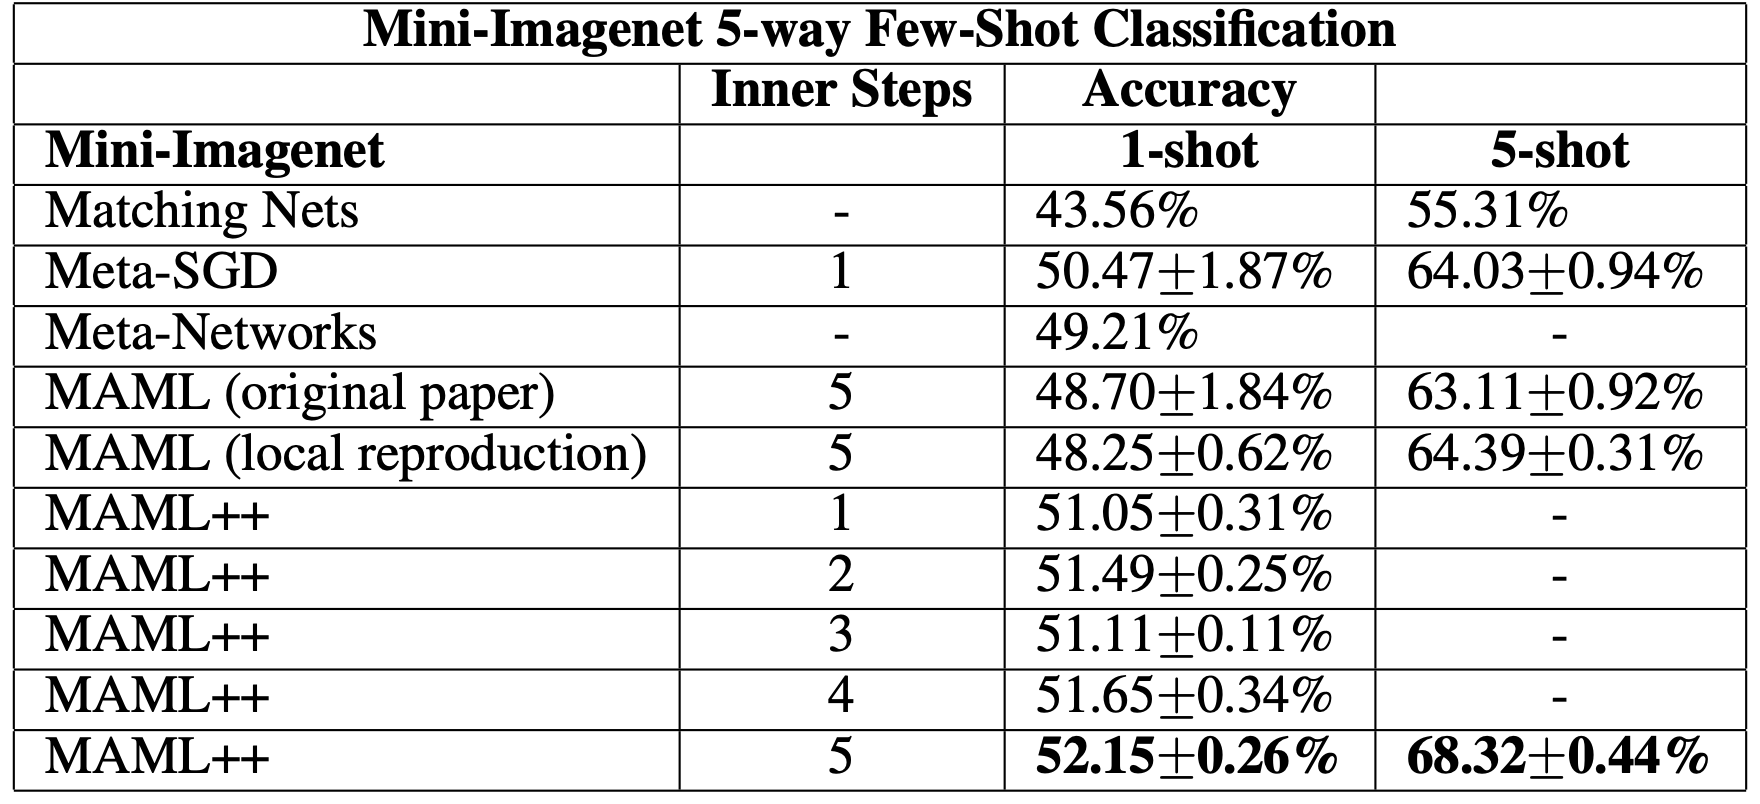
\includegraphics[scale=0.35]{images/table2.png}
        \caption{MAML++ Mini-Imagenet Results}
        \label{fig:enter-label}
    \end{figure}
\end{frame}

\begin{frame}{Results}
    \begin{figure}{}
        \centering
        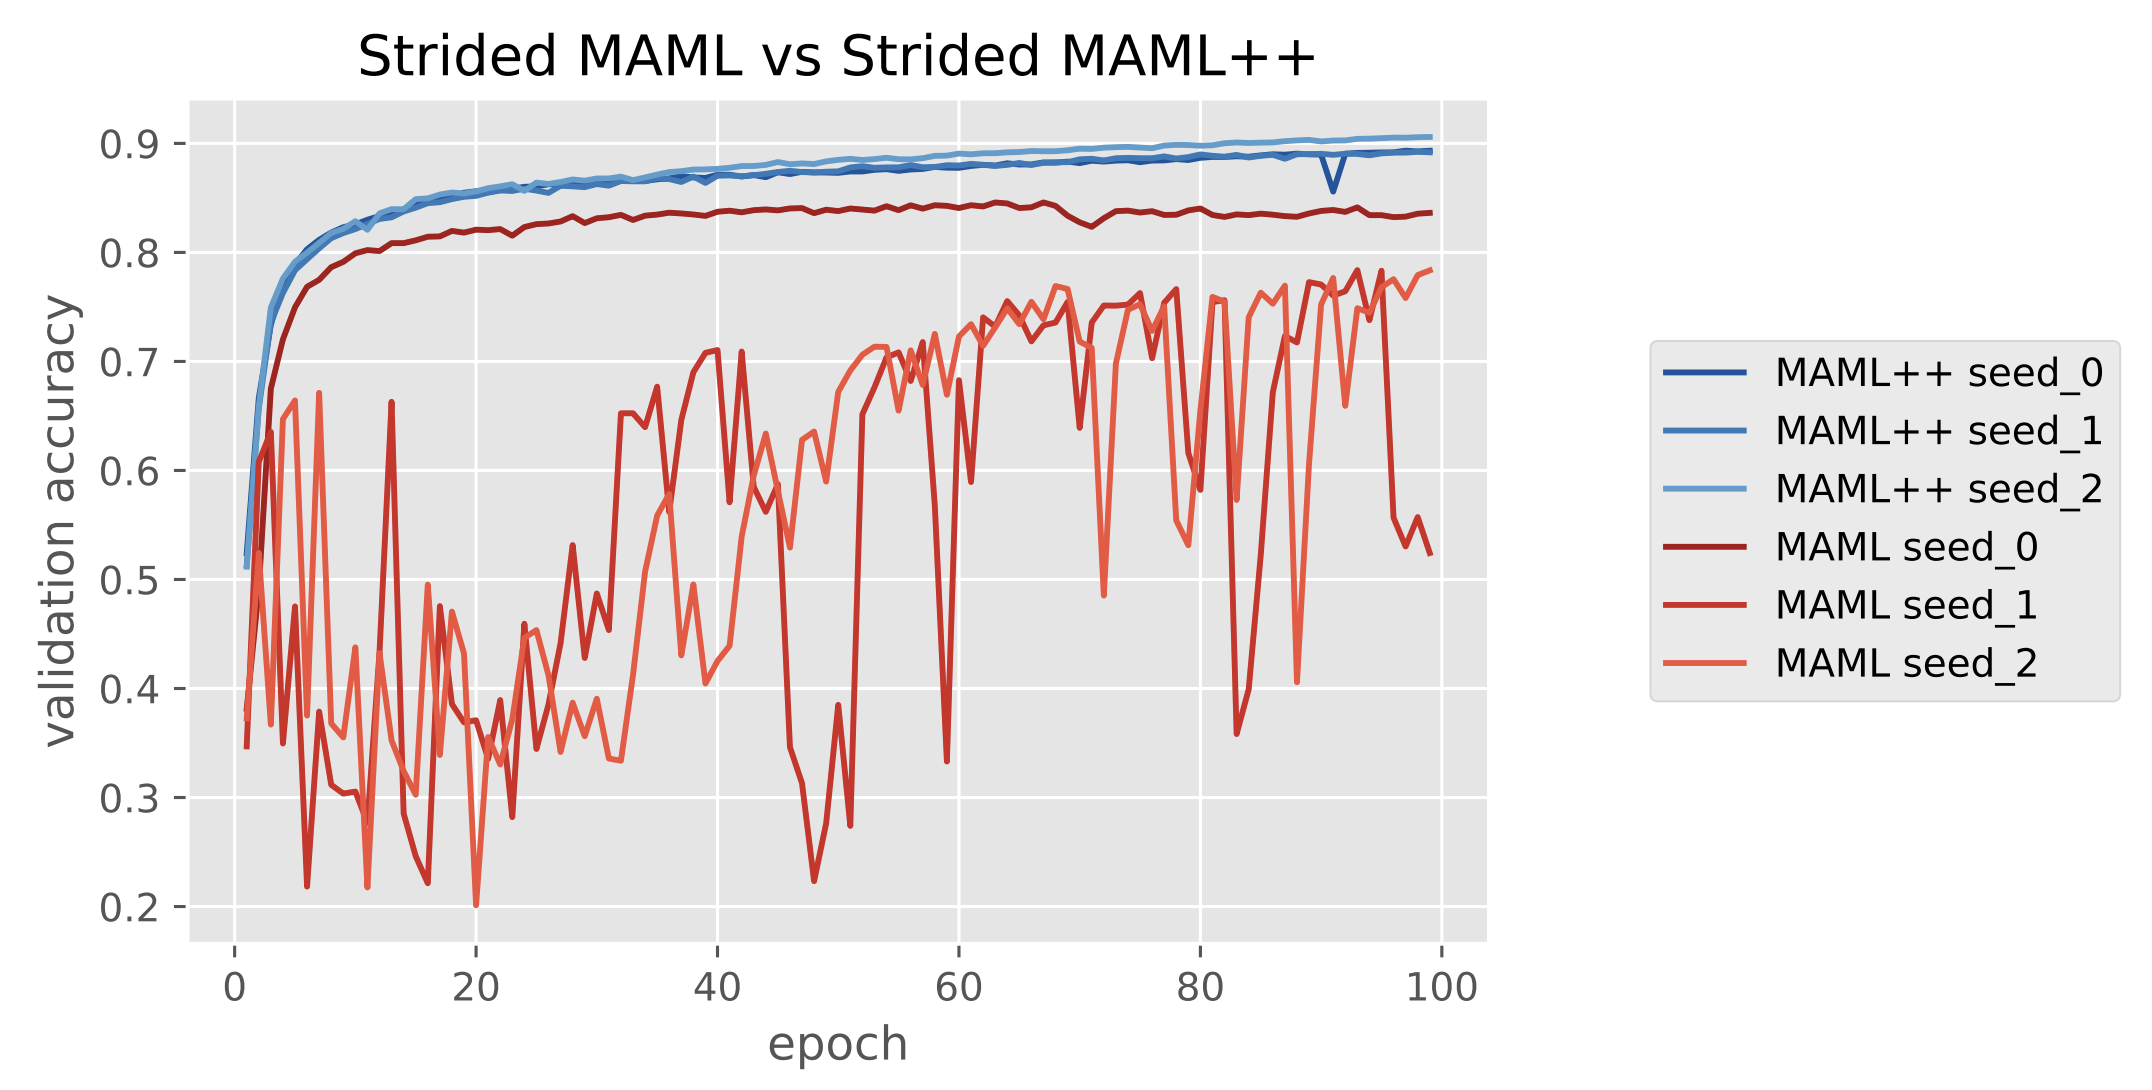
\includegraphics[scale=0.3]{images/figure1.png}
        \caption{Stabilizing MAML: This figure illustrates 3 seeds of the original strided MAML vs strided MAML++. One can see that 2 out of 3 seeds with the original strided MAML seem to become unstable and erratic, whereas all 3 of the strided MAML++ models seem to consistently converge very fast, to much higher generalization accuracy without any stability issues}
        \label{fig:enter-label}
    \end{figure}
\end{frame}

\begin{frame}{Literature}
    \begin{enumerate}
        \item \textbf{Main article} \href{https://arxiv.org/pdf/1810.09502.pdf} 
        {How To Train Your MAML}
    \end{enumerate}
\end{frame}

\end{document}